%%% FP2001.tex 05.10.2000 - Vesa Kolhinen <vesa.kolhinen@phys.jyu.fi>
%%% Original version:
%%% FP2000.tex 12.10.1999 - Eero Noponen <eero.noponen@hut.fi>
%%%
%%%
%%%
%%% Sample LaTeX file for the abstracts for the Proceedings of the
%%% Annual Meeting of the Finnish Physical Society.

\documentclass[12pt]{article}
\usepackage{fp2009}
\usepackage[T1]{fontenc}
\usepackage[latin1]{inputenc}
\usepackage{hyperref}

%%% Remove the following line if Times font is unavailable.
\usepackage{times}

%%% The following line is required if the document contains figures.
\usepackage{graphicx}

%%% The following line is for LaTeX 2.09.
%\documentstyle[FP2001,12pt]{article}

\begin{document}

%%%
%%% The title of the abstract is given here as \title{TITLE TEXT}.
%%%
\title{INCL/ABLA INTRA-NUCLEAR CASCADE MODELS IN GEANT4 9.2}
%\title{INCL INTRA-NUCLEAR CASCADE MODEL IN GEANT9.2} % even more narrow scope?
%\title{INCL/ABLA INTRA-NUCLEAR CASCADE MODEL UPDATES}


%%%
%%% The list of authors; underline the name of the author who is responsible
%%% for the presentation of the paper.
%%%
\underline{P. Kaitaniemi}$^{1, 2}$ A. Heikkinen$^1$ 

%%%
%%% The address.
%%%
$^1$~P.O.Box 64 (Gustaf H\"allstr\"omin katu 2), FIN-00014 University of Helsinki, Finland\\
email: pekka.kaitaniemi@gmail.com

$^2$~CEN-Saclay, CEA-IRFU/SPhN, 91 191 Gif sur Yvette, France

%%%
%%% Body text begins here.
%%%
We discuss the status of INCL intra-nuclear cascade and ABLA fission/de-excitation codes
in the latest relase of the detector simulation toolkit Geant4 9.2 \cite{pk09aCollaboration}.
The INCL model is well established for targets heavier than Aluminium
and projectile energies from $\sim$ 150 MeV up to 2.5 GeV $\sim$ 3 GeV \cite{pk08bProceedings}. 
We present a new Geant4 physics list prepared for nuclear physics applications
in the domain dominated by spallation.

%Improvements of the physics models are foreseen for the treatment of light targets (Carbon - Oxygen)
%and light ion beams (up to Carbon) and will be discussed.
%Outside this domain (light nuclei and energies down to 20-30 MeV)
%the model can be tried but the capabilities have yet to be established.
%such as spallation reactions in Accelerator Driven Systems.
%%% The following minipage structures are needed to position the figure
%%% beside the text paragraph.
%%% For a standard figure environment, see the example below.

\begin{minipage}{6cm}
Validity of the Geant4 physics list is demonstrated from the perspective of accelerator driven systems
and EURISOL project, especially with the neutron double differential cross sections and residual
nuclei production.
An example application utilizing the physics list is introduced.
%
Finally, an ongoing work to improve of the physics models for the treatment of 
light targets (Carbon - Oxygen) and light ion beams (up to Carbon) are discussed.
Finally, an ongoing work to improve of the physics models for the treatment of 
light targets (Carbon - Oxygen) and light ion beams (up to Carbon) (Fig.~1) are discussed.
\end{minipage}
\hfill
\begin{minipage}{9cm}
%
\includegraphics[width=1.0\textwidth]{logo.eps}
%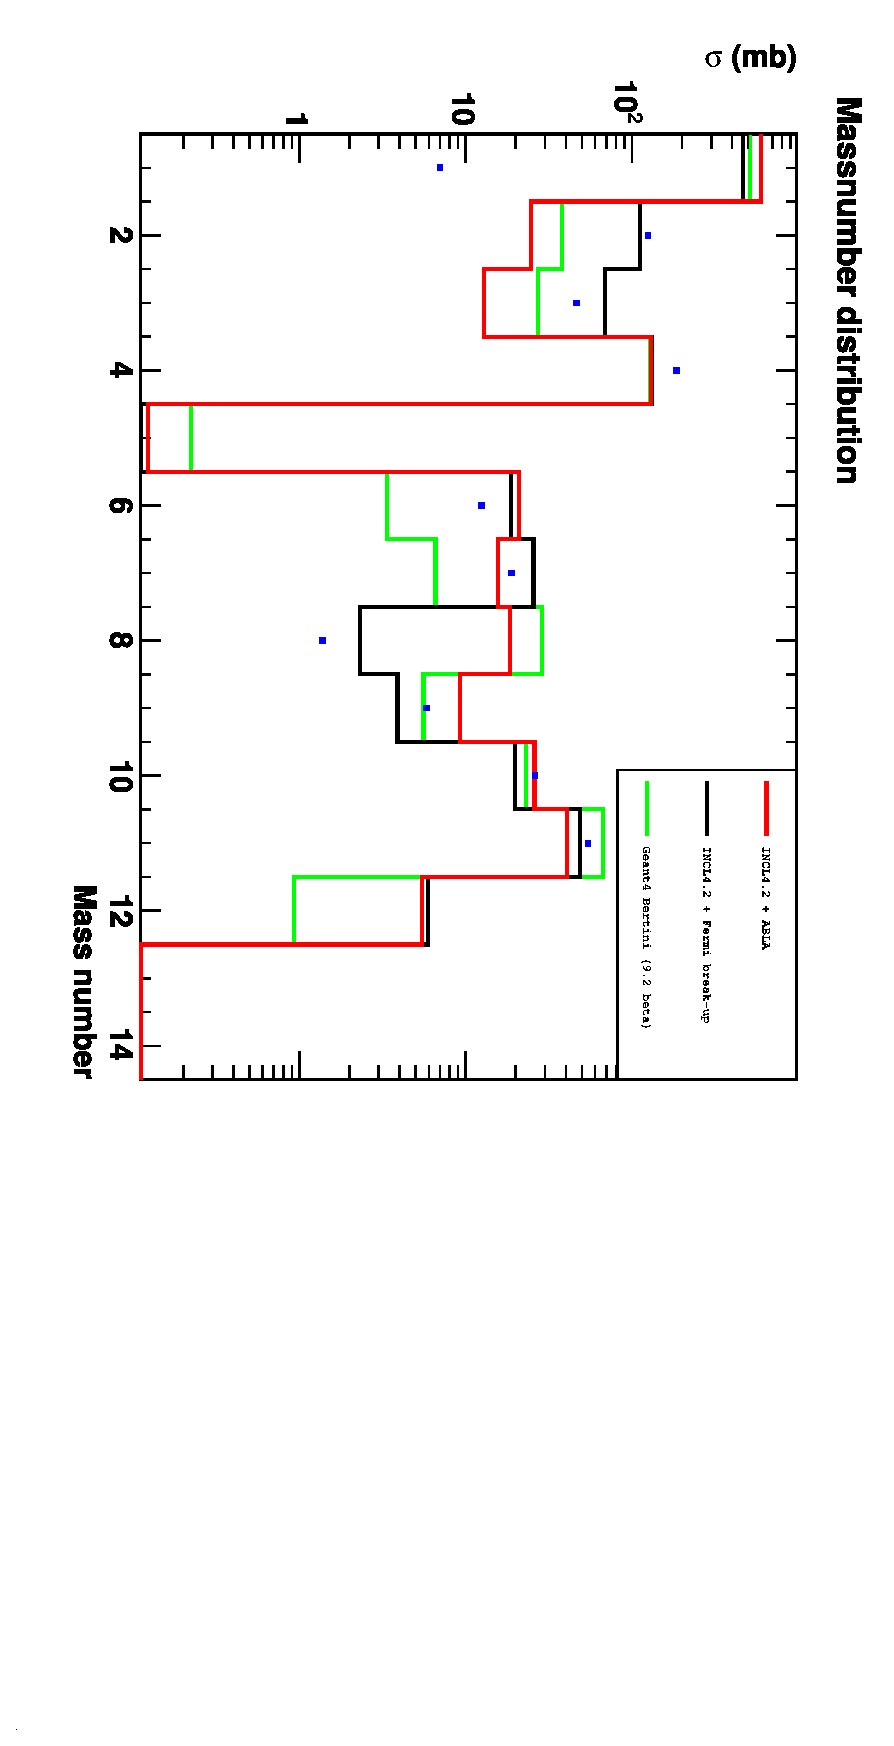
\includegraphics[angle=90,scale=0.5]{masses.eps}
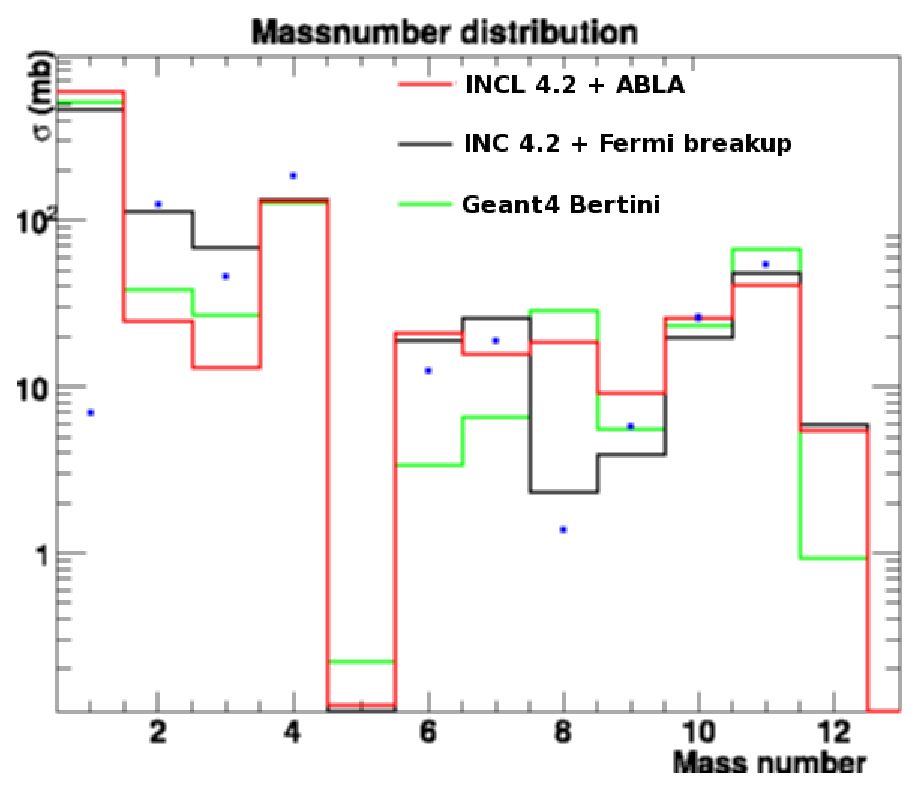
\includegraphics[scale=0.59]{masses2.eps}
{\bf Fig.~1}~Mass of the isotopes produced in reaction p(1 GeV) + $^{12}C$.
INCL/ABLA, INCL with Fermi break-up, 
and Geant4 Bertini simulations are compared with experimental data points from \cite{carbone}.
\end{minipage}


%%%
%%% A more typical Figure.
%%%
%\begin{figure}[!h]
%\centering
\includegraphics[width=4cm]{logo.eps}
%\caption{Mallikuva.}
%\end{figure}

%\begin{figure}

%\end{figure}

%%%
%%% The bibliography: the references are listed here.
%%%
\begin{thebibliography}{9}

\bibitem{pk09aCollaboration}
P. Kaitaniemi and A. Heikkinen with Geant4 Collaboration
\href{http://www.geant4.org}{http://www.geant4.org}

\bibitem{pk08aProceedings}
P. Kaitaniemi and A. Heikkinen,  
{\em INCL4 cascade and ABLA evaporation codes in Geant4},
Proceedings of the XLII annual conference of the Finnish Physical Society, 
                 March 27-29 2008, Turku, Finland. 
                 Report Series in Physics L 31, University of Turku, 2008.

\bibitem{pk08bProceedings}
A. Heikkinen, P. Kaitaniemi, and A. Boudard,
Implementation of INCL4 cascade and ABLA evaporation codes in Geant4,
Journal of Physics: Conference Series 119 (2008) 032024, 
{\sf [doi:10.1088/1742-6596/119/3/032024]}

\bibitem{carbone}
D.L. Olson et al
Factorization of fragment-production cross sections in relativistic heavy-ion collisions,
Phys. Rev. C28, 1602 (1983)
{\sf [doi:10.1103/PhysRevC.28.1602]}

%\href{http://link.aps.org/abstract/PR/v108/p1175}{Fysiikan Lehti 108
%(1957) 1175}.
\end{thebibliography}

\end{document}
